\documentclass[hyperref, a4paper]{article}

\usepackage{geometry}
\usepackage{float}
\usepackage{titling}
\usepackage{titlesec}
% No longer needed, since we will use enumitem package
% \usepackage{paralist}
\usepackage{enumitem}
\usepackage{footnote}
% \usepackage{enumerate}
\usepackage{amsmath, amssymb, amsthm}
\usepackage{mathtools}
\usepackage{bbm}
\usepackage{cite}
\usepackage{graphicx}
\usepackage{subcaption}
\usepackage{physics}
\usepackage{tensor}
\usepackage{siunitx}
\usepackage{booktabs}
\usepackage[version=4]{mhchem}
\usepackage{tikz}
\usepackage{xcolor}
\usepackage{listings}
\usepackage{autobreak}
\usepackage[ruled, vlined, linesnumbered]{algorithm2e}
\usepackage{xr-hyper}
\usepackage[colorlinks,unicode]{hyperref} % , linkcolor=black, anchorcolor=black, citecolor=black, urlcolor=black, filecolor=black
\usepackage[most]{tcolorbox}
\usepackage{prettyref}

% Page style
\geometry{left=3.18cm,right=3.18cm,top=2.54cm,bottom=2.54cm}
\titlespacing{\paragraph}{0pt}{1pt}{10pt}[20pt]
\setlength{\droptitle}{-5em}
\preauthor{\vspace{-10pt}\begin{center}}
\postauthor{\par\end{center}}

% More compact lists 
\setlist[itemize]{itemindent=17pt, leftmargin=1pt}

% Math operators
\DeclareMathOperator{\timeorder}{\mathcal{T}}
\DeclareMathOperator{\diag}{diag}
\DeclareMathOperator{\legpoly}{P}
\DeclareMathOperator{\primevalue}{P}
\DeclareMathOperator{\sgn}{sgn}
\newcommand*{\ii}{\mathrm{i}}
\newcommand*{\ee}{\mathrm{e}}
\newcommand*{\const}{\mathrm{const}}
\newcommand*{\suchthat}{\quad \text{s.t.} \quad}
\newcommand*{\argmin}{\arg\min}
\newcommand*{\argmax}{\arg\max}
\newcommand*{\normalorder}[1]{: #1 :}
\newcommand*{\pair}[1]{\langle #1 \rangle}
\newcommand*{\fd}[1]{\mathcal{D} #1}
\DeclareMathOperator{\bigO}{\mathcal{O}}
\DeclareMathOperator{\object}{Ob}
\DeclareMathOperator{\morphism}{Hom}

% TikZ setting
\usetikzlibrary{arrows,shapes,positioning}
\usetikzlibrary{arrows.meta}
\usetikzlibrary{decorations.markings}
\tikzstyle arrowstyle=[scale=1]
\tikzstyle directed=[postaction={decorate,decoration={markings,
    mark=at position .5 with {\arrow[arrowstyle]{stealth}}}}]
\tikzstyle ray=[directed, thick]
\tikzstyle dot=[anchor=base,fill,circle,inner sep=1pt]

% Algorithm setting
% Julia-style code
\SetKwIF{If}{ElseIf}{Else}{if}{}{elseif}{else}{end}
\SetKwFor{For}{for}{}{end}
\SetKwFor{While}{while}{}{end}
\SetKwProg{Function}{function}{}{end}
\SetArgSty{textnormal}

\newcommand*{\concept}[1]{{\textbf{#1}}}

\newrefformat{fig}{Figure~\ref{#1}}

% Embedded codes
\lstset{basicstyle=\ttfamily,
  showstringspaces=false,
  commentstyle=\color{gray},
  keywordstyle=\color{blue}
}

% Color boxes
\tcbuselibrary{skins, breakable, theorems}
\newtcbtheorem[number within=section]{warning}{Warning}%
  {colback=orange!5,colframe=orange!65,fonttitle=\bfseries, breakable}{warn}
\newtcbtheorem[number within=section]{note}{Note}%
  {colback=green!5,colframe=green!65,fonttitle=\bfseries, breakable}{note}

\title{Quantum Optics, Homework 3}
\author{Jinyuan Wu}

\begin{document}

\maketitle

\begin{figure}
    \centering
    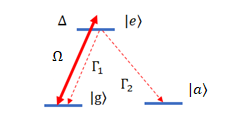
\includegraphics[width=0.4\textwidth]{fig1.png}
    \caption{A three-level $\Lambda$ system}
    \label{fig:sys-1}
\end{figure}

\paragraph{Stochastic wave function of a $\Lambda$ system} \prettyref{fig:sys-1} is a three-level $\Lambda$ system.
(a) Write down the effective Hamiltonian and quantum jump operators for \prettyref{fig:sys-1}.
(b) Suppose $\ket*{\psi_\text{s}(t=0)} = \ket*{\text{g}}$. Describe how the wave function evolves using pseudocode.
(c) Consider a case in which there is no quantum jump in $0 < t < t_0$. Find the time evolution of the 
wave function and the scattering rate 
\begin{equation}
    \gamma_1 = \expval*{C_1^\dagger C_1}{\psi_\text{s}}, \quad \gamma_2 = \expval*{C_2^\dagger C_2}{\psi_\text{s}}.
\end{equation}

\paragraph{Solution} \begin{itemize}
\item[(a)] The effective Hamiltonian is
\begin{equation}  
    \begin{aligned}
        H_\text{eff} &= - \hbar \Delta \dyad{\text{e}} + \left( \frac{1}{2} \hbar \Omega \dyad{\text{e}}{\text{g}} + \text{h.c.} \right) - \frac{\ii \hbar}{2} (C_1^\dagger C_1 + C_2^\dagger C_2) \\
        &= - \hbar (\Delta + \ii \Gamma / 2) \dyad{\text{e}} + \hbar (\Omega \dyad{\text{e}}{\text{g}} + \text{h.c.}) / 2,
    \end{aligned}
    \label{eq:h-eff-1}
\end{equation}  
where the quantum jump operators are 
\begin{equation}
    C_1 = \sqrt{\Gamma_1} \dyad*{\text{a}}{\text{e}}, \quad C_2 = \sqrt{\Gamma_2} \dyad*{\text{g}}{\text{e}},
\end{equation}
and 
\begin{equation}
    \Gamma = \Gamma_1 + \Gamma_2.
\end{equation}

\item[(b)] The time evolution can be described using the following algorithm.
 
\begin{algorithm*}[H]

    \DontPrintSemicolon
    \SetAlgoLined

    \SetKwInOut{Input}{input}
    \SetKwInOut{Output}{output}
    \Input{Time step $\Delta t$, maximal time $t_0$}

    Initialize an array $\{ \ket*{\psi_\text{s}(t)} \}_{t=n \Delta t}$ of wave functions with $t_0 / \Delta t$ elements  \;
    \For{$t \in 0 : \Delta t : t_0$}{
        Pick up a uniformly distributed random number $x$ between $0$ and $1$ \;
        $P_\text{g} \leftarrow \Delta t \expval*{C_1^\dagger C_1}{\psi_\text{s}(t)}$ \;
        $P_\text{a} \leftarrow \Delta t \expval*{C_2^\dagger C_2}{\psi_\text{s}(t)}$ \;
        \tcp*[h]{jumping to $\ket*{\text{g}}$} \;
        \uIf{
            $0 < x < P_\text{g}$}{
            $\ket*{\psi_\text{s}(t + \Delta t)} \leftarrow \text{normalized } C_1 \ket*{\psi_\text{s}(t)} $ \;
        }
        \tcp*[h]{jumping to $\ket*{\text{a}}$} \;
        \uElseIf{
            $P_\text{g} < x < P_\text{g} + P_\text{a}$
        }{
            $\ket*{\psi_\text{s}(t + \Delta t)} \leftarrow \text{normalized } C_2 \ket*{\psi_\text{s}(t)} $ \;
        }
        \tcp*[h]{evolution according to the effective Hamiltonian} \;
        \Else{
            $\ket*{\psi_\text{s}(t + \Delta t)} \leftarrow \text{normalized } \ket*{\psi_\text{s}(t)} + \frac{\Delta t}{\ii \hbar} H_\text{eff} \ket*{\psi_\text{s}(t)} $ \;
        }
    }
    
  \end{algorithm*}
\item[(c)] The wave function in this case evolves purely according to $H_\text{eff}$. Since Schrödinger equation
is linear, we can leave the normalization to the end of our calculation. Note that \eqref{eq:h-eff-1} actually
does not contain $\ket*{\text{a}}$ explicitly, nor does the initial state $\ket*{\text{g}}$. Therefore we can 
work in the two-level system spanned by $\ket*{\text{e}}$ and $\ket*{\text{g}}$. The effective Hamiltonian is 
\begin{equation}
    H_\text{eff} = \hbar \pmqty{0 & \Omega^* / 2 \\ \Omega / 2 & - (\Delta + \ii \Gamma / 2)},
\end{equation}
where we let $\ket*{\text{g}}$ be the first component and $\ket*{\text{e}}$ the second. We have the decomposition 
\begin{equation}
    H_\text{eff} = - \frac{\hbar}{2} (\Delta + \ii \Gamma) + \frac{\hbar}{2} \vb*{\Omega} \cdot \vb*{\sigma}, \quad 
    \vb*{\Omega} = (\Omega_\text{r}, \Omega_\text{i}, \Delta + \ii \Gamma / 2).
    \label{eq:h-eff-1-decomp}
\end{equation}
Note here we cannot ``shift the energy zero point'' to reshape the Hamiltonian into $\vb*{\Omega} \cdot \vb*{\sigma}$, because 
the value damping rate has physical meaning. Applying \eqref{eq:h-eff-1-decomp} on $\ket*{\text{g}}$, we have 
\[
    \begin{aligned}
        \ee^{- \ii H_\text{eff} t / \hbar} \ket*{\text{g}} &= 
        \ee^{\ii t (\Delta + \ii \Gamma / 2) / 2} \ee^{- \ii t \vb*{\Omega} \cdot \vb*{\sigma} / 2} \ket*{\text{g}} \\
        &= \ee^{- \Gamma t / 4} \ee^{\ii \Delta t / 2} \left( \sigma^0 \cos \frac{\abs*{\vb*{\Omega}} t}{2}  
        - \frac{\ii \vb*{\Omega} \cdot \vb*{\sigma}}{\abs*{\vb*{\Omega}}} \sin \frac{\abs*{\vb*{\Omega}} t}{2} \right) \ket*{\text{g}} \\
        &= \ee^{- \Gamma t / 4} \ee^{\ii \Delta t / 2} \left(\cos \frac{\abs*{\vb*{\Omega}} t}{2} \ket*{\text{g}} - \left( \frac{\Omega_\text{r}}{\abs*{\vb*{\Omega}}} \ket*{\text{e}} + \frac{\ii \Omega_\text{i}}{\abs*{\vb*{\Omega}}} \ket*{\text{e}} + \frac{\Delta + \ii \Gamma / 2}{\abs*{\vb*{\Omega}}} \ket*{\text{g}} \right) \ii \sin \frac{\abs*{\vb*{\Omega}} t}{2} \right)  ,
    \end{aligned}
\] 
where 
\begin{equation}
    \abs*{\vb*{\Omega}} = \sqrt{\abs*{\Omega}^2 + \Delta^2 - \Gamma^2 / 4 + \ii \Delta \Gamma}.
\end{equation}
\begin{note*}{}{}
    Note that here $\abs*{\vb*{n}}$ is defined as $\sqrt{\vb*{n} \cdot \vb*{n}}$ instead of 
    $\sqrt{\vb*{n}^* \cdot \vb*{n}}$, because to make 
    \[
        \ee^{\ii \alpha \vb*{n} \cdot \vb*{\sigma}} = \sigma^0 \cos \alpha + \ii \vb*{n} \cdot \vb*{\sigma} \sin \alpha
    \]
    hold, it is required that 
    \[
        (\vb*{n} \cdot \vb*{\sigma})^2 = \sigma^0,
    \]
    which is equivalent to $\vb*{n} \cdot \vb*{n} = 1$, considering $\acomm*{\sigma^i}{\sigma^j} = 0$ 
    when $i \neq j$. What is important here, therefore, is $\vb*{n} \cdot \vb*{n}$.
\end{note*}
Therefore we have (we have omitted the complex factors, since they will be canceled by normalization anyway) 
\begin{equation}
    \ket*{\psi_\text{s}(t)} \propto \left( \cos \frac{\abs*{\vb*{\Omega}} t}{2} - \ii \frac{\Delta + \ii \Gamma / 2}{\abs*{\vb*{\Omega}}} \sin \frac{\abs*{\vb*{\Omega}} t}{2}  \right) \ket*{\text{g}} - \frac{\ii \Omega}{\abs*{\vb*{\Omega}}} \sin \frac{\abs*{\vb*{\Omega}} t}{2} \ket*{\text{e}},
\end{equation}
and after normalization it is 

\item

\end{itemize}

\paragraph{}

\paragraph{Cesium atom} 

\paragraph{EIT-assisted giant Kerr effect} The "lambda"-system composed of $|\text{a}\rangle,|\text{e}\rangle,|\text{b}\rangle \quad$ is further coupled to excited state $|\text{c}\rangle$, as in Fig. 1. We consider the situation of EIT-resonance: $\delta=0$. We further consider atomic state to be initially in $|\psi(t=0)\rangle=|\mathrm{a}\rangle$, and weak-excitation limit is satisfied $\left(\left|\Omega_{1}\right|\right.$ small "enough").
3a) Write down the effective Hamiltonian for this problem for $\delta=0$
3b) Obtain the approximate stochastic wavefunction in its steady state $\left|\widetilde{\psi_\text{S}}\right\rangle=|\text{a}\rangle+$ ${c}_{\mathrm{e}}|\text{e}\rangle+c_\text{b}|\text{b}\rangle+c_\text{c}|\text{c}\rangle$ such that $\mathrm{H}_{\mathrm{eff}}\left|\psi_{\mathrm{S}}\right\rangle \approx 0$

\paragraph{Solution} \begin{itemize}
\item[(a)]  
\end{itemize}

\paragraph{}

\end{document}